% Created with jtex v.1.0.13
\documentclass{article}
\PassOptionsToPackage{short, nodayofweek}{datetime}


% Start Curvenote Definitions

% Pass Options Section
% base
\PassOptionsToPackage{normalem}{ulem}
\PassOptionsToPackage{utf8}{inputenc}

% template
\PassOptionsToPackage{framemethod=TikZ}{mdframed}
\PassOptionsToPackage{x11names, svgnames}{xcolor}

%%% PACKAGES

% base
\usepackage{inputenc}
\usepackage{url}
\usepackage{graphicx}
\usepackage{adjustbox}
\usepackage{amssymb}
\usepackage{amsfonts}
\usepackage{amsmath}
\usepackage{enumitem}
\usepackage{nicefrac}
\usepackage{booktabs}
\usepackage{microtype}
\usepackage{hyperref}
\usepackage{ulem}
\usepackage{enumitem}
\usepackage{float}
\usepackage{datetime}
\usepackage{xkeyval}
\usepackage{framed}
\usepackage{doi}

% template
\usepackage{natbib}
\usepackage{fancyvrb}
\usepackage{mdframed}
\usepackage{xcolor}

%%%


%%%% Setup Section

% base
\graphicspath{{.}}
% template
\sloppy
\newenvironment{aside}{\begin{framed}}{\end{framed}}
\newmdenv[linewidth=2pt,linecolor=CornflowerBlue,topline=false,bottomline=false,rightline=false,leftline=true,skipabove=20,skipbelow=20,leftmargin=20,rightmargin=20]{callout}
\newfloat{code}{thp}{loc}
\floatname{code}{Program}
\raggedbottom
\bibliographystyle{abbrvnat}
\setcitestyle{authoryear,open={(},close={)},semicolon,aysep={,}}

% End Curvenote Definitions




% colors for hyperlinks
\hypersetup{colorlinks=true, allcolors=blue}
\hypersetup{
pdftitle={\@title},
pdfsubject={},
pdfauthor={\@author},
pdfkeywords={},
addtopdfcreator={Written in Curvenote}
}

\usepackage{curvenote}

\title{Informations}

\newdate{articleDate}{4}{2}{2024}
\date{\displaydate{articleDate}}

\author{\bfseries Jean-Marc Pouchoulon\mdseries\\Enseignant IUT Béziers\\}

\begin{document}

\maketitle
\keywords{CI/CD Cloud DevOps Gitlab}

\textbf{Compétences ciblées:}

-- Coordonner des infrastructures modulaires

-- Accompagner le développement d'applications

\textbf{Objectifs et problématique professionnelle :}

Le professionnel R\&T spécialisé en Développement Système et Cloud fait évoluer des applications existantes au sein de
son entreprise en développant de nouvelles fonctionnalités. L'application pouvant déjà être en production et utilisée par des
collaborateurs ou des clients, il ne peut donc pas interrompre l'usage qui en est fait. Il intègre ses apports en utilisant une
approche CI/CD (intégration continue, déploiement continu). Cette approche permet de tester les nouvelles fonctionnalités
en s'assurant de leurs compatibilités avec l'existant avant de planifier leurs mises à disposition auprès des utilisateurs sans
interruption de service.

\textbf{Descriptif générique :}

Le professionnel DevCloud met en œuvre la chaîne CI/CD d'une application structurée en microservices, intervient et surveille
les différentes étapes du cycle de développement (dont la gestion des erreurs et des messages). Afin d'assurer le développement des fonctionnalités, il applique la démarche suivante :

-- la mise en place de la chaîne d'intégration continue (CI) et ses différents tests ;

-- la mise en place de la chaîne de développement continue (CD) incluant la génération du livrable applicatif sous la forme
d'un conteneur et le déploiement automatique de l'application avec ses améliorations ;

-- la vérification de la santé du code incluant le monitoring de l'application, un système d'alertes, la prise en compte de la
sécurité à tous les niveaux de l'application et la gestion des messages (incluant les logs) renvoyés par l'application ;

-- la planification du déploiement avec le nettoyage des bases de données de l'orchestrateur, l'automatisation du déploie-
ment en tenant compte de l'activité et la gestion d'un backup ;

-- la gestion des agents de messages pour la communication entre deux microservices (sous la forme d'une file FIFO par
exemple).

\textbf{Apprentissages critiques :}

-- AC34.01DevCloud | Concevoir, administrer et superviser une infrastructure Cloud

-- AC34.02DevCloud | Orchestrer les ressources Cloud

-- AC34.03DevCloud | Investiguer sur les incidents et les résoudre afin d'améliorer la qualité et la fiabilité des infrastructures

-- AC35.01DevCloud | Adopter les pratiques de pilotage de projet

-- AC35.02DevCloud | Concevoir, gérer et sécuriser un environnement de microservices

-- AC35.03DevCloud | Gérer son infrastructure comme du code

-- AC35.04DevCloud | Gérer une chaîne d'intégration et/ou de déploiement continu

\section{Informations}

\begin{framed}
\textbf{Note}\\
Ce document est écrit avec Myst Markdown qui améliore les possibilités de Markdown. Vous devrez aussi utiliser ce format pour vos rendus.
\end{framed}

Remplir de jolis tableaux de compétences :kissing:

Je peux faire des maths aussi

$E=mc^2$

mettre des images de chats:

\begin{figure}[!htbp]
\centering
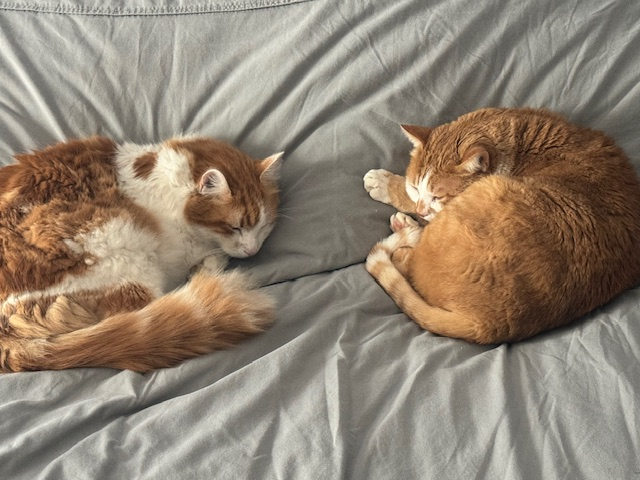
\includegraphics[width=0.625\linewidth]{files/chats-00ce8bd69eb8aebbc2204cc6d332458f.jpg}
\caption*{Ils sont beaux mes chats non ? {\textasciitilde}{\textasciitilde}2 points \textbf{en plus} si vous dites yes sir{\textasciitilde}{\textasciitilde} !}
\end{figure}

On peut aussi \newline
``breaker'' le texte \newline
à la ``latex''
avec {\textbackslash}~(que vous ne voyez pas ici)

Avez-vous bien

\begin{itemize}
\item compris ?
\item pas compris ?
\end{itemize}

C'est du markdow\textsuperscript{2}!

Plus avoir plus d'exemples allez sur \href{https://myst-parser.readthedocs.io/en/latest/}{Myst Markdown}

Dans un premier temps Il vous est demandé d'automatiser de rendre accessible ces logs.

Dans un second temps d'en automatiser l'exploitation afin de produire:

\begin{itemize}
\item des rapports de sécurité (bilan synthétique des attaques et des tentatives d'attaques, nombre de virus) sous forme d'une application web déployé dans un cluster Kubernetes.
\item des repository de listes noires accessibles sur gitlab et github et mis à jour automatiquement.  Vous générerez automatiquement des scripts de pare-feu pour NetFilter/iptables-nftables.
\end{itemize}

Le projet sera collaboratif  et les scripts seront versionnés sur un repository git. Le build et le déploiement des scripts se fera sur un serveur de CI/CD (gitlab ou github).
Vous utiliserez un serveur mis à disposition par votre entreprise pour le déploiement de votre solution

+mattermost
%%%%%%%%%%%%%%%%%%%%%%%%%%%%%%%%%%%%%%%%%%%%%%%%%%
%%%%%%%%%%%%%%  acronyms & glossary  %%%%%%%%%%%%%
\printglossaries
%%%%%%%%%%%%%%%%%%%%%%%%%%%%%%%%%%%%%%%%%%%%%%%%%%

\end{document}
